\chapter{Estruturas de Mercado, Barreiras de Entrada e Aglomerações Produtivas}
\tagAV{AV1 (30\%)}\ \tagTerritorio

\begin{capObjetivos}
Ao concluir este capítulo, você será capaz de:
\begin{itemize}[leftmargin=1.4em, itemsep=2pt]
  \item Distinguir as quatro estruturas clássicas de mercado (concorrência perfeita, monopólio, oligopólio e concorrência monopolística) quanto ao poder de precificação e à dinâmica de entrada.
  \item Aplicar o Modelo das Cinco Forças de Porter (1979; 1980) e as estratégias genéricas (liderança em custo, diferenciação e foco) à inserção competitiva de EBTs.
  \item Analisar barreiras econômicas, tecnológicas e regulatórias à entrada e à saída de mercados.
  \item Calcular e interpretar o Índice Herfindahl--Hirschman ($\text{HHI}$) e a variação de concentração ($\Delta \text{HHI}$) em operações de fusão ou entrada territorial.
  \item Explicar a transição da firma isolada para a Eficiência Coletiva em Arranjos Produtivos Locais (APLs), contrapondo a noção de espaço neutro ao território socialmente construído.
\end{itemize}
\end{capObjetivos}

\begin{capRevisao}
Para acompanhar a modelagem deste capítulo, relembre três fundamentos:
\begin{enumerate}[leftmargin=1.4em, itemsep=2pt]
  \item \textbf{Participação de mercado (\textit{market share}):} fração $s_i = q_i / Q_{\text{tot}}$ (em proporção de $0$ a $1$ ou em pontos percentuais de $0$ a $100$) detida pela firma $i$ nas vendas totais do setor relevante.
  \item \textbf{Economias de escala:} redução do custo médio unitário ($\text{CMe} = C_{\text{tot}} / Q$) à medida que o volume produzido $Q$ cresce, diluindo os custos fixos.
  \item \textbf{Custos afundados (\textit{sunk costs}):} investimentos específicos já realizados que não podem ser recuperados caso a empresa encerre suas atividades no setor.
\end{enumerate}
\end{capRevisao}

\etapa{3}{Estruturas de Mercado, Estratégia Competitiva e Eficiência Coletiva}

\begin{boxSimbolo}[Vocabulário Conceitual e Notação do Capítulo]
\begin{tabularx}{\linewidth}{@{}l X@{}}
  \toprule
  \textbf{Símbolo / Termo} & \textbf{Significado Analítico e Unidade} \\
  \midrule
  $s_i$ & Participação de mercado (\textit{market share}) da empresa $i$, expressa em \% ($0$ a $100$) ou proporção ($0$ a $1$). \\
  $\text{HHI}$ & Índice Herfindahl--Hirschman de concentração de mercado ($0$ a $10.000$ na escala percentual). \\
  $\Delta \text{HHI}$ & Variação do $\text{HHI}$ decorrente da fusão entre duas firmas $A$ e $B$ ($\Delta \text{HHI} = 2 s_A s_B$). \\
  $CR_k$ & Razão de concentração das $k$ maiores empresas do mercado ($CR_k = \sum_{i=1}^k s_i$). \\
  EME & Escala Mínima Eficiente: menor nível de produção em que o custo médio de longo prazo atinge seu mínimo. \\
  APL & Arranjo Produtivo Local: aglomeração territorial de agentes econômicos, políticos e sociais com foco em conjunto específico de atividades. \\
  EC & Eficiência Coletiva (Schmitz): vantagem competitiva derivada de economias externas locais somadas à ação conjunta deliberada. \\
  \bottomrule
\end{tabularx}
\end{boxSimbolo}

\section{Estruturas Clássicas de Mercado e Poder de Precificação}

A capacidade de uma Empresa de Base Tecnológica capturar valor depende diretamente da estrutura do mercado em que ingressa. Na teoria microeconômica, os mercados organizam-se em quatro arquétipos principais conforme o número de ofertantes, o grau de diferenciação do produto e a altura das barreiras à entrada. Na \textbf{Concorrência Perfeita}, um grande número de compradores e vendedores atomizados negocia produto homogêneo sob informação simétrica e livre entrada e saída, de modo que nenhuma firma controla o preço e todas atuam como tomadoras de preço ($P = \text{CMg}$ no equilíbrio de longo prazo). No extremo oposto encontra-se o \textbf{Monopólio}, caracterizado por um único ofertante de um bem ou serviço sem substitutos próximos, protegido por barreiras legais como patentes e concessões, pelo controle de insumo essencial ou por monopólio natural decorrente de custos fixos elevados frente à demanda, o que permite à firma definir preço ou quantidade e apropriar-se de rendas monopolistas.

Entre esses dois polos situam-se as estruturas mais frequentes na trajetória de EBTs. No \textbf{Oligopólio}, um pequeno número de grandes empresas domina a oferta e gera forte interdependência estratégica nas decisões de preço, capacidade e P\&D, compondo a estrutura típica de setores \textit{Mark II} como telecomunicações, semicondutores e defensivos agrícolas. Já na \textbf{Concorrência Monopolística}, numerosas firmas ofertam produtos diferenciados por marca, \textit{design}, funcionalidade ou atendimento localizado sob barreiras moderadas, conferindo a cada firma poder de mercado local sobre seu nicho, ainda que lucros extraordinários atraiam novos entrantes no longo prazo.

\section{Cinco Forças de Porter, Estratégias Genéricas e Barreiras}

Michael Porter (1979; 1980) estruturou a análise da atratividade setorial ao mostrar que a rentabilidade de uma indústria resulta da interação simultânea de cinco forças competitivas. Esse campo de forças combina a \textbf{rivalidade entre concorrentes existentes} e a \textbf{ameaça de novos entrantes} com a pressão exercida pela \textbf{ameaça de produtos ou serviços substitutos}, pelo \textbf{poder de barganha dos compradores} e pelo \textbf{poder de barganha dos fornecedores}.

Para posicionar-se de maneira defensável diante dessas forças, Porter (1980) propôs três \textbf{estratégias genéricas}. A \textbf{liderança em custo total} apoia-se em escala e eficiência operacional para ofertar preços menores, ao passo que a \textbf{diferenciação} constrói atributos únicos percebidos pelo cliente que justificam um prêmio de preço. A terceira via corresponde ao \textbf{foco}, voltado à atuação concentrada em um segmento, nicho tecnológico ou recorte territorial específico, operando tanto pela via do custo quanto pela diferenciação.

As \textbf{barreiras à entrada} determinam quão difícil é para uma nova EBT ingressar em um setor, envolvendo economias de escala exigidas na entrada, diferenciação e lealdade à marca, requisitos elevados de capital inicial, custos de mudança para o comprador, acesso restrito a canais de distribuição, desvantagens de custo independentes de escala (como patentes e curvas de aprendizagem) e regulação governamental (licenças sanitárias, ambientais ou registros no MAPA/ANVISA). De modo complementar, as \textbf{barreiras à saída} decorrem de ativos altamente especializados, custos fixos rescisórios, inter-relações estratégicas e compromissos sociais que mantêm empresas operando mesmo com margens negativas, acirrando a rivalidade do setor.

\begin{boxFormula}[Índice Herfindahl--Hirschman ($\text{HHI}$) de Concentração de Mercado]
\textbf{Origem.} Desenvolvido independentemente por Albert O. Hirschman (1945) e Orris C. Herfindahl (1950), é o indicador padrão utilizado por autoridades antitruste como o CADE (Brasil) e o DOJ/FTC (EUA) para medir concentração horizontal.

\textbf{Variáveis.} O cálculo considera o número total de empresas atuantes no mercado relevante $N$, a participação de mercado da empresa $i$ em pontos percentuais $s_i$ ($0 \le s_i \le 100$, com $\sum_{i=1}^N s_i = 100$) e as participações percentuais $s_A$ e $s_B$ de duas empresas candidatas a fusão ou aquisição.

\textbf{Fórmulas passo a passo:}
\[
\text{HHI} = \sum_{i=1}^{N} s_i^2
\qquad\qquad
\Delta \text{HHI} = \text{HHI}_{\text{pós}} - \text{HHI}_{\text{pré}} = (s_A + s_B)^2 - (s_A^2 + s_B^2) = 2 s_A s_B
\]

\textbf{Critérios interpretativos (escala $0$ a $10.000$).} Mercados com $\text{HHI} < 1.500$ são classificados como não concentrados, indicando estrutura competitiva. Quando $1.500 \le \text{HHI} \le 2.500$, observa-se concentração moderada, ao passo que valores de $\text{HHI} > 2.500$ caracterizam mercados altamente concentrados, correspondendo a oligopólio restrito ou a monopólio no limite de $\text{HHI} = 10.000$.

\textbf{Exemplo rápido.} Um mercado com $4$ empresas de participações $40\%$, $30\%$, $20\%$ e $10\%$ tem $\text{HHI} = 40^2 + 30^2 + 20^2 + 10^2 = 1.600 + 900 + 400 + 100 = 3.000$ (altamente concentrado). Se as duas menores ($20\%$ e $10\%$) se fundirem, $\Delta \text{HHI} = 2 \times 20 \times 10 = 400$, elevando o índice para $3.400$.
\end{boxFormula}

\section{Da Firma Isolada à Eficiência Coletiva em APLs e Território Social}

O modelo porteriano tradicional analisa a firma individual em confronto com forças externas. Contudo, pequenas e médias empresas tecnológicas enfrentam desvantagens severas de escala quando atuam isoladas. Hubert Schmitz (1995; 1999) evidenciou que a aglomeração geográfica em \textbf{Arranjos Produtivos Locais (APLs)} permite superar tais limitações por meio da \textbf{Eficiência Coletiva}, resultante da combinação de dois componentes complementares.

O primeiro componente abrange as \textbf{economias externas marshallianas} (não intencionais ou passivas), que reúnem benefícios gerados espontaneamente pela concentração espacial de firmas similares por meio da formação de um mercado de trabalho especializado, da atração de fornecedores dedicados de insumos, manutenção e serviços técnicos e dos transbordamentos tecnológicos e informacionais (\textit{spillovers}). O segundo componente corresponde à \textbf{ação conjunta deliberada} (intencional ou ativa), expressa na cooperação consciente entre empresas e instituições locais em arranjos horizontais (consórcios de compra, laboratórios compartilhados, certificação coletiva e feiras) ou verticais (programas de qualificação de fornecedores e codesenvolvimento tecnológico).

\begin{boxConceito}[Contraponto Crítico: Espaço Neutro vs. Território Socialmente Construído]
Na economia espacial neoclássica e em leituras simplificadas de clusters, o espaço é tratado como um \textbf{plano neutro e isotrópico}, no qual a localização ótima resulta apenas da minimização de custos de transporte e fatores. Em contraste, a geografia econômica crítica e a abordagem territorial latino-americana entendem o \textbf{território como construção social, histórica e política}. A simples aglomeração produtiva exige governança ativa para gerar eficiência coletiva, pois relações assimétricas de poder entre grandes compradores e microprodutores, desconfiança institucional, captura de consórcios por elites locais ou precarização do trabalho podem bloquear a cooperação e transformar um polo produtivo em enclave extrativo sem desenvolvimento endógeno.
\end{boxConceito}

Essa passagem da concorrência atomizada para a cooperação territorializada reorganiza o posicionamento estratégico das pequenas firmas frente aos grandes concorrentes. Conforme ilustra a Figura~\ref{fig:porter_eficiencia_coletiva}, a articulação entre economias externas marshallianas e ação conjunta deliberada desloca a firma isolada da vulnerabilidade estrutural das Cinco Forças de Porter para um patamar superior de competitividade sistêmica em Arranjos Produtivos Locais.

\begin{figure}[H]
  \centering
  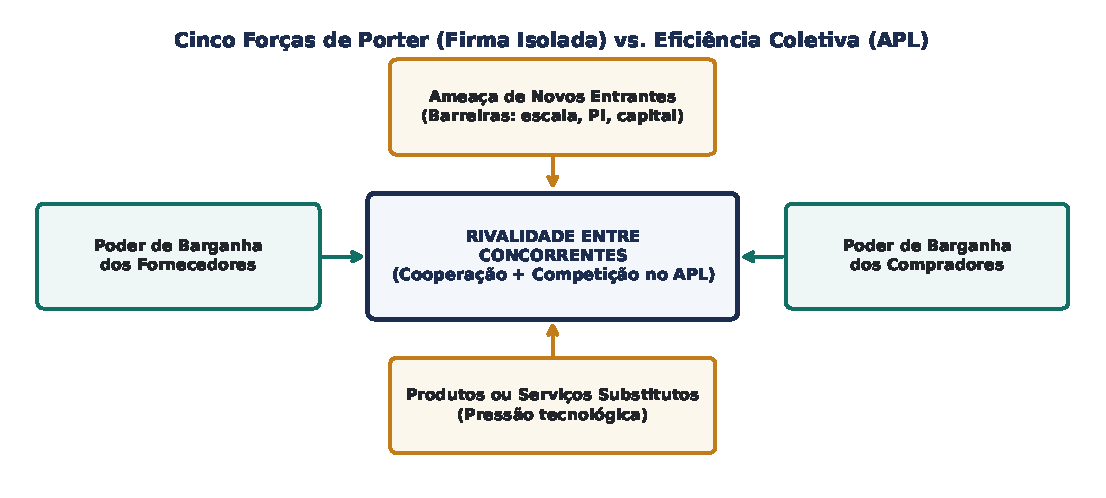
\includegraphics[width=0.94\textwidth]{figures/fig02_porter_eficiencia_coletiva.pdf}
  \caption{Transição analítica entre a firma isolada sob pressão das Cinco Forças de Porter e o ganho de Eficiência Coletiva (economias externas marshallianas + ação conjunta deliberada) em Arranjos Produtivos Locais.}
  \label{fig:porter_eficiencia_coletiva}
\end{figure}

\etapa{4}{Estudos de Caso e Aplicações Passo a Passo}

\begin{boxExemplo}{1}{Cálculo do Índice HHI, $CR_4$ e Impacto de Fusão em AgTechs}
\passoEnunciado{O mercado regional de softwares de gestão para agricultura familiar no Nordeste é atendido por cinco empresas com as seguintes participações nas vendas anuais: Empresa A ($35\%$), Empresa B ($25\%$), Empresa C ($20\%$), Empresa D ($12\%$) e Empresa E ($8\%$). A Empresa B propõe adquirir integralmente a Empresa D.}
\passoDados{$s_A = 35$; $s_B = 25$; $s_C = 20$; $s_D = 12$; $s_E = 8$ (soma $= 100\%$). Operação proposta: fusão B + D.}
\passoPedido{Calcular o $CR_4$ e o $\text{HHI}$ antes da fusão, a variação $\Delta \text{HHI}$ e o novo $\text{HHI}$ pós-fusão, classificando o grau de concentração segundo os critérios antitruste.}
\passoMetodo{Cálculo direto de $CR_4 = \sum_{i=1}^4 s_i$, $\text{HHI}_{\text{pré}} = \sum s_i^2$, $\Delta \text{HHI} = 2 s_B s_D$ e $\text{HHI}_{\text{pós}} = \text{HHI}_{\text{pré}} + \Delta \text{HHI}$.}
\passoContas{
  \begin{enumerate}[leftmargin=1.4em, itemsep=2pt]
    \item Razão de concentração das quatro maiores pré-fusão ($CR_4$):
    \[
    CR_4 = 35 + 25 + 20 + 12 = 92\%
    \]
    \item Cálculo do $\text{HHI}_{\text{pré}}$:
    \[
    \text{HHI}_{\text{pré}} = 35^2 + 25^2 + 20^2 + 12^2 + 8^2 = 1.225 + 625 + 400 + 144 + 64 = 2.458
    \]
    \item Variação $\Delta \text{HHI}$ com a fusão B + D ($s_{B+D} = 25 + 12 = 37\%$):
    \[
    \Delta \text{HHI} = 2 \times 25 \times 12 = 600
    \]
    \item Conferência direta do $\text{HHI}_{\text{pós}}$:
    \[
    \text{HHI}_{\text{pós}} = 35^2 + 37^2 + 20^2 + 8^2 = 1.225 + 1.369 + 400 + 64 = 3.058
    \]
    \[
    \text{Verificação:} \quad 2.458 + 600 = 3.058
    \]
  \end{enumerate}
}
\passoResposta{$CR_4 = 92\%$; $\text{HHI}_{\text{pré}} = 2.458$ (moderadamente concentrado); $\Delta \text{HHI} = 600$; $\text{HHI}_{\text{pós}} = 3.058$ (altamente concentrado).}
\passoVerificacao{Como o $\text{HHI}_{\text{pós}}$ ultrapassa $2.500$ com um salto $\Delta \text{HHI} = 600$ (muito acima do limiar típico de alerta de $200$ pontos), a operação gera risco anticompetitivo relevante, podendo elevar preços de licenciamento para cooperativas locais e criar barreiras à entrada de novas startups regionais.}
\end{boxExemplo}

\begin{boxExemplo}{2}{Matriz Ponderada das Cinco Forças de Porter para EBT Solar}
\passoEnunciado{Uma EBT de microinversores solares inteligentes avalia ingressar no segmento comercial de pequeno porte no Semiárido. Sua equipe atribuiu pesos estratégicos às Cinco Forças de Porter (soma $= 1{,}00$) e notas de pressão competitiva de $1$ (pressão muito baixa/favorável) a $5$ (pressão muito alta/desfavorável): Rivalidade ($w_1 = 0{,}30$, nota $4{,}0$); Novos Entrantes ($w_2 = 0{,}20$, nota $3{,}0$); Substitutos ($w_3 = 0{,}15$, nota $2{,}0$); Poder dos Compradores ($w_4 = 0{,}20$, nota $3{,}5$); Poder dos Fornecedores de chips asiáticos ($w_5 = 0{,}15$, nota $4{,}5$).}
\passoDados{Pesos $w = (0{,}30; 0{,}20; 0{,}15; 0{,}20; 0{,}15)$ e notas $N = (4{,}0; 3{,}0; 2{,}0; 3{,}5; 4{,}5)$.}
\passoPedido{Calcular o Índice Global de Pressão Setorial ($P_{\text{Porter}}$) e indicar qual estratégia genérica de Porter é mais defensável.}
\passoMetodo{Média aritmética ponderada $P_{\text{Porter}} = \sum_{j=1}^5 w_j N_j$.}
\passoContas{
  \begin{enumerate}[leftmargin=1.4em, itemsep=2pt]
    \item Contribuição ponderada de cada força:
    \[
    w_1 N_1 = 0{,}30 \times 4{,}0 = 1{,}20
    \]
    \[
    w_2 N_2 = 0{,}20 \times 3{,}0 = 0{,}60
    \]
    \[
    w_3 N_3 = 0{,}15 \times 2{,}0 = 0{,}30
    \]
    \[
    w_4 N_4 = 0{,}20 \times 3{,}5 = 0{,}70
    \]
    \[
    w_5 N_5 = 0{,}15 \times 4{,}5 = 0{,}675
    \]
    \item Soma ponderada total:
    \[
    P_{\text{Porter}} = 1{,}20 + 0{,}60 + 0{,}30 + 0{,}70 + 0{,}675 = 3{,}475\text{ (em escala de 1 a 5)}
    \]
  \end{enumerate}
}
\passoResposta{$P_{\text{Porter}} = 3{,}475$ (pressão competitivo-estrutural moderada a alta). A estratégia mais indicada é o \textbf{Foco com Diferenciação} em monitoramento térmico e assistência técnica local.}
\passoVerificacao{Competir por liderança em custo contra grandes fabricantes asiáticos (nota $4{,}5$ nos fornecedores e $4{,}0$ na rivalidade) inviabilizaria a EBT regional. O foco diferenciado (equipamento adaptado a altas temperaturas e suporte local ágil) reduz a sensibilidade a preço dos compradores e cria custos de mudança.}
\end{boxExemplo}

\begin{boxExemplo}{3}{Barreiras à Entrada e Escala Mínima Eficiente (EME) no Território}
\passoEnunciado{Para operar uma planta de envase asséptico de polpas funcionais da caatinga (como umbu e maracujá-do-mato) com certificação de exportação, a tecnologia impõe custos fixos anuais de $\text{CF} = \reais{900.000}$/ano e custo variável unitário de $\text{CVu} = \reais{4{,}00}$/litro. A demanda regional total do mercado endereçável é de $Q_{\text{merc}} = 600.000$ litros/ano, e o preço médio praticado no mercado é de $P = \reais{10{,}00}$/litro. Uma planta é considerada competitiva quando atinge a Escala Mínima Eficiente (EME) onde o custo médio unitário não ultrapassa $\reais{7{,}00}$/litro.}
\passoDados{$\text{CF} = \reais{900.000}$/ano; $\text{CVu} = \reais{4{,}00}$/L; $\text{CM}_{\text{alvo}} = \reais{7{,}00}$/L; $Q_{\text{merc}} = 600.000$ L/ano.}
\passoPedido{Calcular o volume correspondente à EME, o percentual do mercado regional que uma única planta precisa capturar para atingir a EME e o número máximo teórico de plantas eficientes comportadas pelo mercado.}
\passoMetodo{Custo médio $\text{CM}(Q) = \frac{\text{CF}}{Q} + \text{CVu}$. Igualar $\text{CM}(Q) = \text{CM}_{\text{alvo}}$ para encontrar $Q_{\text{EME}}$ e calcular a fração $s_{\text{EME}} = Q_{\text{EME}} / Q_{\text{merc}}$.}
\passoContas{
  \begin{enumerate}[leftmargin=1.4em, itemsep=2pt]
    \item Equação da Escala Mínima Eficiente:
    \[
    \frac{900.000}{Q_{\text{EME}}} + 4{,}00 = 7{,}00 \implies \frac{900.000}{Q_{\text{EME}}} = 3{,}00
    \]
    \[
    Q_{\text{EME}} = \frac{900.000}{3{,}00} = 300.000\text{ litros/ano}
    \]
    \item Participação de mercado exigida pela EME:
    \[
    s_{\text{EME}} = \frac{300.000}{600.000} \times 100\% = 50{,}0\%
    \]
    \item Número máximo de plantas na EME:
    \[
    N_{\max} = \frac{Q_{\text{merc}}}{Q_{\text{EME}}} = \frac{600.000}{300.000} = 2\text{ plantas}
    \]
  \end{enumerate}
}
\passoResposta{$Q_{\text{EME}} = 300.000$ L/ano; cada entrante precisa capturar $50\%$ do mercado regional; o território comporta no máximo $2$ plantas nessa escala.}
\passoVerificacao{O resultado demonstra como economias de escala formam uma barreira natural à entrada que induz estrutura oligopolista ($2$ firmas, $\text{HHI}$ mínimo de $50^2 + 50^2 = 5.000$). Uma alternativa territorial inteligente é a formação de uma agroindústria cooperativa compartilhada (ação conjunta) para diluir os $\reais{900.000}$ fixos entre dezenas de produtores.}
\end{boxExemplo}

\begin{boxExemplo}{4}{Quantificação da Eficiência Coletiva em Arranjo Produtivo Local}
\passoEnunciado{Considere uma microempresa isolada de confecção técnica/têxtil que produz $10.000$ peças/ano a um custo unitário base de $\reais{50{,}00}$/peça (total de $\reais{500.000}$/ano). Ao integrar-se a um APL estruturado no interior do estado, a empresa obtém dois ganhos distintos: (1) por economias externas marshallianas (proximidade de oficinas de manutenção e mão de obra treinada), reduz perdas e tempo ocioso em $8\%$ sobre o custo base; (2) por ação conjunta deliberada (consórcio de compras de tecido tecnológico e laboratório compartilhado de controle de qualidade), reduz em mais $12\%$ o custo já ajustado pelas economias externas. O consórcio cobra uma anuidade associativa fixa de $\reais{12.000}$/ano.}
\passoDados{$Q = 10.000$ peças; $\text{CM}_0 = \reais{50{,}00}$/peça; redução passiva $d_1 = 8\%$; redução ativa $d_2 = 12\%$; taxa associativa $F_{\text{assoc}} = \reais{12.000}$/ano.}
\passoPedido{Calcular o custo unitário após economias externas, o custo após ação conjunta (antes e depois da anuidade) e o ganho líquido anual em Eficiência Coletiva.}
\passoMetodo{Aplicação sequencial dos fatores $(1 - d_1)$ e $(1 - d_2)$, seguida da adição do custo fixo associativo diluído ($F_{\text{assoc}} / Q$).}
\passoContas{
  \begin{enumerate}[leftmargin=1.4em, itemsep=2pt]
    \item Custo unitário após economias externas marshallianas:
    \[
    \text{CM}_1 = 50{,}00 \times (1 - 0{,}08) = 50{,}00 \times 0{,}92 = \reais{46{,}00}\text{/peça}
    \]
    \item Custo unitário após ação conjunta deliberada (antes da anuidade):
    \[
    \text{CM}_2 = 46{,}00 \times (1 - 0{,}12) = 46{,}00 \times 0{,}88 = \reais{40{,}48}\text{/peça}
    \]
    \item Custo total anual no APL incluindo anuidade de $\reais{12.000}$:
    \[
    C_{\text{tot,APL}} = (10.000 \times 40{,}48) + 12.000 = 404.800 + 12.000 = \reais{416.800}\text{/ano}
    \]
    \item Custo unitário final líquido e economia total anual:
    \[
    \text{CM}_{\text{final}} = \frac{416.800}{10.000} = \reais{41{,}68}\text{/peça}
    \]
    \[
    \text{Ganho líquido anual} = 500.000 - 416.800 = \reais{83.200}\text{/ano} \quad (\text{redução líquida de } 16{,}64\%)
    \]
  \end{enumerate}
}
\passoResposta{$\text{CM}_1 = \reais{46{,}00}$, $\text{CM}_2 = \reais{40{,}48}$, $\text{CM}_{\text{final}} = \reais{41{,}68}$/peça e ganho líquido de $\reais{83.200}$/ano ($16{,}64\%$).}
\passoVerificacao{O exercício ilustra o núcleo da teoria de Schmitz: estar apenas geograficamente próximo gera $\reais{40.000}$ de economia passiva ($8\%$), mas a governança da ação conjunta acrescenta mais $\reais{43.200}$ líquidos após pagar a anuidade. O território socialmente organizado produz competitividade inacessível à firma isolada.}
\end{boxExemplo}

\begin{boxExemplo}{5}{Barreiras à Saída e Custos Afundados (\textit{Sunk Costs})}
\passoEnunciado{Uma empresa tradicional de processamento mineral investiu $\reais{2.000.000}$ em um forno rotativo dedicado cuja venda como sucata renderia apenas $\reais{250.000}$, além de enfrentar multa ambiental e rescisões trabalhistas de $\reais{350.000}$ caso encerre a operação hoje. No próximo ano, projeta-se receita de $\reais{1.100.000}$ e custos operacionais correntes de $\reais{1.220.000}$ (prejuízo operacional de $\reais{120.000}$).}
\passoDados{Investimento histórico $= \reais{2.000.000}$; valor de revenda $V_{\text{rev}} = \reais{250.000}$; custo de encerramento $C_{\text{enc}} = \reais{350.000}$; resultado operacional anual projetado $= -\reais{120.000}$.}
\passoPedido{Calcular o custo afundado (\textit{sunk cost}), o saldo líquido de saída imediata e explicar por que a firma pode optar por permanecer operando no curto prazo, agravando a rivalidade setorial.}
\passoMetodo{Cálculo do custo irrecuperável ($\text{SC} = I_0 - V_{\text{rev}}$) e comparação entre o fluxo de saída imediata ($V_{\text{rev}} - C_{\text{enc}}$) e a perda operacional de permanecer ($-\reais{120.000}$).}
\passoContas{
  \begin{enumerate}[leftmargin=1.4em, itemsep=2pt]
    \item Custo afundado do ativo dedicado:
    \[
    \text{SC} = 2.000.000 - 250.000 = \reais{1.750.000}
    \]
    \item Fluxo líquido de caixa caso decida sair hoje:
    \[
    F_{\text{saída}} = V_{\text{rev}} - C_{\text{enc}} = 250.000 - 350.000 = -\reais{100.000}
    \]
    \item Comparação com a manutenção da operação por mais $1$ ano (aguardando recuperação de preços): se permanecer, perde $\reais{120.000}$ no ano, mas preserva a opção de recuperar demanda; se sair, desembolsa $\reais{100.000}$ líquidos imediatamente e perde definitivamente o ativo produtivo.
  \end{enumerate}
}
\passoResposta{Custo afundado de $\reais{1.750.000}$ e saldo de saída imediata de $-\reais{100.000}$.}
\passoVerificacao{Em mercados com altas barreiras à saída (ativos específicos e altos encargos de encerramento), firmas deficitárias permanecem produzindo para cobrir parte dos custos ou aguardar reversão de ciclo, mantendo excesso de capacidade e intensificando a guerra de preços prevista por Porter.}
\end{boxExemplo}

\etapa{5}{Armadilhas Conceituais e Erros Mais Comuns}

\begin{boxErro}[Erro 1: Confundir Concentração de Mercado ($\text{HHI}$) com Lucro Garantido]
Um $\text{HHI}$ superior a $2.500$ indica alta concentração entre ofertantes atuais, mas não garante rentabilidade automática se a ameaça de substitutos ou o poder de barganha dos compradores (Forças 3 e 4 de Porter) forem extremos. Um monopólio local de transporte fluvial pode ter $\text{HHI} = 10.000$ e margens comprimidas pela concorrência do transporte rodoviário substituto.
\end{boxErro}

\begin{boxErro}[Erro 2: Misturar Escalas no Cálculo do Índice HHI]
Calcular o $\text{HHI}$ somando participações em proporção ($0{,}40^2 + 0{,}60^2 = 0{,}52$) e compará-lo diretamente com a faixa regulatória de $1.500$ a $2.500$ (que usa escala percentual de $0$ a $100$) é um erro clássico. Na escala percentual, $\text{HHI} \in (0, 10.000]$; na escala decimal, $\text{HHI}_{\text{dec}} \in (0, 1]$, sendo a conversão $\text{HHI} = 10.000 \times \text{HHI}_{\text{dec}}$.
\end{boxErro}

\begin{boxErro}[Erro 3: Reduzir APL a Simples Aglomeração Geográfica]
Muitos projetos territoriais chamam qualquer conjunto de empresas próximas de APL com eficiência coletiva. Sem ação conjunta deliberada (governança compartilhada, compras coletivas, inovação cooperativa), a simples proximidade espacial gera no máximo economias marshallianas passivas e pode degenerar em guerra predatória de preços entre vizinhos.
\end{boxErro}

\begin{boxErro}[Erro 4: Tentar Competir por Liderança em Custo em Nichos de Baixa Escala]
Startups e EBTs iniciantes frequentemente tentam vencer incumbentes baixando preços antes de atingir a Escala Mínima Eficiente (EME). Sem volume para diluir custos fixos de P\&D e estrutura, a estratégia de liderança em custo destrói o caixa inicial; o caminho viável na entrada costuma ser diferenciação ou foco territorial/tecnológico.
\end{boxErro}

\etapa{6}{Lista de Exercícios (15 Questões Graduadas)}

\subsection*{Bloco A: Conceituais e Básicos (Questões 1 a 5)}

\begin{enumerate}[leftmargin=1.6em, itemsep=6pt]
  \item Compare concorrência perfeita, concorrência monopolística e oligopólio quanto à diferenciação do produto, ao número de firmas e à capacidade de influenciar o preço de mercado.
  \espacoResolucao[1.8cm]

  \item Liste as Cinco Forças Competitivas de Porter (1979) e explique por que um alto poder de barganha de fornecedores especializados reduz a rentabilidade potencial de uma EBT.
  \espacoResolucao[1.8cm]

  \item Um mercado de serviços de geoprocessamento com drones é dividido igualmente entre $5$ empresas ($20\%$ cada). Calcule o $\text{HHI}$ desse mercado e classifique-o segundo as faixas usuais ($<1.500$, $1.500$--$2.500$, $>2.500$).
  \espacoResolucao[1.8cm]

  \item Diferencie barreiras à entrada de barreiras à saída, citando dois exemplos concretos de cada uma no contexto de empreendimentos industriais ou agroindustriais.
  \espacoResolucao[1.8cm]

  \item Defina \textit{Eficiência Coletiva} segundo Hubert Schmitz, explicando a diferença entre economias externas marshallianas e ação conjunta deliberada.
  \espacoResolucao[1.8cm]
\end{enumerate}

\subsection*{Bloco B: Intermediários e Aplicados (Questões 6 a 10)}

\begin{enumerate}[leftmargin=1.6em, itemsep=6pt, resume]
  \item Em um mercado regional de sensores de umidade do solo, quatro empresas detêm as seguintes participações: Firmas 1 ($40\%$), 2 ($30\%$), 3 ($15\%$) e 4 ($15\%$). Calcule o $\text{HHI}$ inicial, a variação $\Delta \text{HHI}$ caso as Firmas 3 e 4 se fundam, e o $\text{HHI}$ final após a fusão.
  \espacoResolucao[2.2cm]

  \item Uma pequena agroindústria de derivados de licuri possui custo fixo anual de $\reais{180.000}$ e custo variável unitário de $\reais{6{,}00}$/kg. Para atingir a Escala Mínima Eficiente (EME), seu custo médio unitário não pode ultrapassar $\reais{10{,}00}$/kg. Calcule a quantidade anual mínima ($Q_{\text{EME}}$) necessária para atingir essa eficiência.
  \espacoResolucao[2.2cm]

  \item Explique como uma EBT do Semiárido pode utilizar a estratégia genérica de \textbf{Foco com Diferenciação} para se proteger da rivalidade de grandes fabricantes multinacionais.
  \espacoResolucao[2.0cm]

  \item Em um APL de apicultura no Nordeste, $20$ associações produzem juntas $100.000$ kg de mel/ano a um custo médio de $\reais{14{,}00}$/kg. Por meio de economias externas locais, o custo cai $5\%$, e por meio de uma casa do mel e envase compartilhados (ação conjunta), cai mais $10\%$ sobre o valor já reduzido, mediante uma taxa anual compartilhada de $\reais{42.000}$ dividida pelo volume total. Calcule o custo unitário final por kg.
  \espacoResolucao[2.2cm]

  \item Discuta o contraponto entre ``espaço neutro'' e ``território socialmente construído'' aplicado à governança de um APL: por que a existência de muitas empresas próximas nem sempre gera inovação cooperativa?
  \espacoResolucao[2.0cm]
\end{enumerate}

\subsection*{Bloco C: Questões Objetivas de Fixação (Questões 11 a 15)}

\begin{enumerate}[leftmargin=1.6em, itemsep=6pt, resume]
  \item No Modelo das Cinco Forças de Porter, a presença de custos de mudança elevados para os clientes que desejam trocar de fornecedor de software atua diretamente para:
  \begin{alternativas}
    \item Reduzir o poder de barganha dos compradores e elevar a barreira à entrada de novos concorrentes.
    \item Eliminar completamente a necessidade de proteção por propriedade intelectual.
    \item Transformar o mercado em uma estrutura de concorrência perfeita com produto homogêneo.
    \item Aumentar o poder de barganha dos fornecedores de matérias-primas básicas.
    \item Reduzir as barreiras à saída das empresas incumbentes.
  \end{alternativas}

  \item Um setor apresenta quatro empresas com participações de $50\%$, $20\%$, $20\%$ e $10\%$. O Índice Herfindahl--Hirschman ($\text{HHI}$) desse mercado é:
  \begin{alternativas}
    \item $1.000$
    \item $2.400$
    \item $3.000$
    \item $3.400$
    \item $4.000$
  \end{alternativas}

  \item Na abordagem de Eficiência Coletiva (Schmitz), constituem exemplos de \textbf{economias externas marshallianas} (passivas) e de \textbf{ação conjunta deliberada} (ativa), respectivamente:
  \begin{alternativas}
    \item Consórcio de exportação e disponibilidade espontânea de mão de obra treinada na região.
    \item Disponibilidade espontânea de fornecedores locais de peças e criação de um laboratório de testes compartilhado pelas empresas.
    \item Guerra de preços entre firmas vizinhas e abertura de filiais em outro continente.
    \item Subsídio federal direto e monopólio legal por patente farmacêutica.
    \item Redução de impostos estaduais e venda isolada de commodities sem certificação.
  \end{alternativas}

  \item Sobre as estratégias genéricas de Porter (1980), assinale a alternativa \textbf{correta}:
  \begin{alternativas}
    \item A liderança em custo exige que a empresa opere sempre com baixos volumes e alta customização artesanal.
    \item A diferenciação busca entregar atributos únicos valorizados pelo comprador que permitam sustentar margem superior à média do setor.
    \item A estratégia de foco consiste em atender simultaneamente todos os segmentos de mercado com o menor preço possível.
    \item O modelo de Porter proíbe que empresas de base tecnológica atuem em nichos regionais.
    \item Barreiras à entrada altas e barreiras à saída baixas representam o pior cenário possível de rentabilidade setorial.
  \end{alternativas}

  \item Na análise de estruturas de mercado, um cenário caracterizado por \textbf{barreiras à entrada baixas} e \textbf{barreiras à saída altas} tende a gerar:
  \begin{alternativas}
    \item Retornos estáveis e elevados no longo prazo, com baixa rivalidade.
    \item Monopólio natural estável com regulação tarifária mínima.
    \item Retornos baixos e voláteis, pois novos concorrentes entram facilmente nos ciclos de alta e permanecem presos em guerras de preços nos ciclos de baixa.
    \item Eliminação imediata de todas as firmas ineficientes sem custos afundados.
    \item Transição automática para a concorrência perfeita sem diferenciação.
  \end{alternativas}
\end{enumerate}

\etapa{7}{Questões de Alta Complexidade (Estilo ANPAD / Pós-Graduação / CT\&I)}

\begin{enumerate}[leftmargin=1.6em, itemsep=8pt]
  \item \textbf{(Estilo ANPAD / Estratégia)} Em um mercado relevante de bioinsumos agrícolas composto por cinco firmas com participações $40\%$, $25\%$, $15\%$, $10\%$ e $10\%$, uma autoridade antitruste analisa duas propostas distintas de fusão: Proposta 1 (união das firmas de $40\%$ e $10\%$) e Proposta 2 (união das firmas de $25\%$ e $15\%$). Considerando a variação $\Delta \text{HHI}$, é correto afirmar que:
  \begin{alternativas}
    \item A Proposta 1 gera $\Delta \text{HHI} = 400$ e a Proposta 2 gera $\Delta \text{HHI} = 375$, portanto a Proposta 2 eleva mais a concentração.
    \item Ambas as propostas resultam no mesmo $\Delta \text{HHI} = 800$, pois envolvem o mesmo número de firmas remanescentes.
    \item A Proposta 1 gera $\Delta \text{HHI} = 800$ e a Proposta 2 gera $\Delta \text{HHI} = 750$, levando o mercado de um $\text{HHI}$ inicial de $2.650$ para $3.450$ ou $3.400$, respectivamente.
    \item O $\text{HHI}$ inicial do mercado é $1.850$ (moderadamente concentrado), tornando ambas as fusões isentas de análise.
    \item A Proposta 2 reduz o $\text{HHI}$ total por equilibrar as participações das duas maiores líderes.
  \end{alternativas}

  \item \textbf{(Estilo Pós-Graduação / Economia Regional)} Sobre a relação entre economias de aglomeração, Eficiência Coletiva e território socialmente construído, analise as assertivas:
  \begin{itemize}[leftmargin=1.2em, itemsep=2pt]
    \item[I.] Economias externas marshallianas explicam ganhos de produtividade decorrentes da proximidade espacial, mas não bastam para explicar respostas coordenadas a choques competitivos externos, que exigem ação conjunta deliberada.
    \item[II.] A concepção de território como espaço neutro garante que toda aglomeração industrial gere distribuição equitativa de renda e cooperação horizontal entre pequenas e grandes firmas.
    \item[III.] Em APLs periféricos, relações assimétricas de governança podem fazer com que grandes compradores externos capturem a maior parte dos ganhos da eficiência coletiva local.
  \end{itemize}
  Está correto o que se afirma em:
  \begin{alternativas}
    \item I, apenas.
    \item II, apenas.
    \item I e III, apenas.
    \item II e III, apenas.
    \item I, II e III.
  \end{alternativas}

  \item \textbf{(Estilo Concurso CT\&I / Desenvolvimento Regional)} Uma EBT de embalagens biodegradáveis de fécula de mandioca enfrenta forte poder de compra de grandes redes varejistas (Força 4 de Porter) e concorrência de embalagens plásticas convencionais (Força 3 de Porter). Para elevar sua defensabilidade estrutural sem entrar em guerra de preços, a decisão mais consistente com o referencial deste capítulo é:
  \begin{alternativas}
    \item Reduzir seus investimentos em P\&D e copiar exatamente o preço do plástico convencional, mesmo abaixo do custo médio.
    \item Buscar diferenciação certificada (compostabilidade e origem territorial) combinada com ação conjunta em consórcio de fornecedores locais para reduzir custos unitários de matéria-prima.
    \item Aumentar deliberadamente suas barreiras à saída imobilizando capital em máquinas sem uso alternativo.
    \item Operar em concorrência perfeita eliminando qualquer registro de patente ou marca própria.
    \item Transferir toda a cadeia produtiva para longe das áreas produtoras de mandioca, tratando a localização como espaço neutro.
  \end{alternativas}
\end{enumerate}

\begin{boxDica}[Contraponto Crítico e Prática Territorial (Conexão AV1 e AV3)]
Na \textbf{AV1}, lembre-se de que o $\text{HHI}$ mede concentração de oferta, enquanto as Cinco Forças de Porter avaliam a pressão estrutural completa do setor. Na \textbf{AV3}, ao desenhar o posicionamento competitivo do seu projeto territorial, evite propor que uma nova EBT vença grandes incumbentes apenas por preço baixo: mostre onde está a barreira de diferenciação, qual é a Escala Mínima Eficiente e como a articulação com um APL local (Eficiência Coletiva) viabiliza custos competitivos.
\end{boxDica}

\clearpage
\etapa{8}{Gabarito Comentado (Questões 1 a 18)}

\begin{boxGabarito}[Respostas Comentadas: Exercícios 1 a 15 e Questões de Alta Complexidade 16 a 18]
\begin{enumerate}[leftmargin=1.6em, itemsep=4pt]
  \item \textbf{Resposta:} Na concorrência perfeita há muitos ofertantes, produto homogêneo e nenhum poder de preço; na concorrência monopolística há muitos ofertantes com produtos diferenciados e poder de preço limitado ao nicho; no oligopólio há poucos grandes ofertantes com forte interdependência estratégica e alto poder de mercado.
  \item \textbf{Resposta:} As cinco forças são: rivalidade entre concorrentes, ameaça de novos entrantes, ameaça de substitutos, poder dos compradores e poder dos fornecedores. Fornecedores concentrados ou detentores de insumos críticos elevam preços e comprimem a margem operacional da EBT.
  \item \textbf{Resposta:} $\text{HHI} = 5 \times 20^2 = 5 \times 400 = 2.000$. Classificação: mercado moderadamente concentrado ($1.500 \le \text{HHI} \le 2.500$).
  \item \textbf{Resposta:} Barreiras à entrada dificultam o ingresso de novas firmas (ex.: exigência de grande capital inicial e registro sanitário/patentes). Barreiras à saída dificultam o encerramento (ex.: equipamentos altamente especializados sem revenda e multas/passivos contratuais ou ambientais).
  \item \textbf{Resposta:} Eficiência Coletiva (Schmitz) é a soma das economias externas marshallianas (ganhos espontâneos de aglomeração: mão de obra, fornecedores e \textit{spillovers}) com a ação conjunta deliberada (cooperação intencional via consórcios, compras ou certificações).
  \item \textbf{Resposta:} $\text{HHI}_{\text{pré}} = 40^2 + 30^2 + 15^2 + 15^2 = 1.600 + 900 + 225 + 225 = 2.950$. $\Delta \text{HHI} = 2 \times 15 \times 15 = 450$. $\text{HHI}_{\text{pós}} = 2.950 + 450 = 3.400$ (ou $40^2 + 30^2 + 30^2 = 3.400$).
  \item \textbf{Resposta:} $\frac{180.000}{Q_{\text{EME}}} + 6{,}00 = 10{,}00 \implies \frac{180.000}{Q_{\text{EME}}} = 4{,}00 \implies Q_{\text{EME}} = 45.000$ kg/ano.
  \item \textbf{Resposta:} Concentrando-se em um nicho geográfico ou funcional específico (ex.: adaptação climática ao Semiárido, assistência técnica local e integração com cooperativas), oferecendo atributos que multinacionais padronizadas não entregam com agilidade, evitando competição direta por escala pura.
  \item \textbf{Resposta:} Após economias externas ($-5\%$): $14{,}00 \times 0{,}95 = \reais{13{,}30}$/kg. Após ação conjunta ($-10\%$): $13{,}30 \times 0{,}90 = \reais{11{,}97}$/kg. Taxa associativa por kg: $42.000 / 100.000 = \reais{0{,}42}$/kg. Custo final $= 11{,}97 + 0{,}42 = \reais{12{,}39}$/kg.
  \item \textbf{Resposta:} O conceito de território socialmente construído mostra que a cooperação depende de confiança, regras de governança e equilíbrio de poder. Onde há desconfiança, assimetria extrema ou captura política, a proximidade física não gera ação conjunta.
  \item \textbf{Gabarito: (A).} Custos de mudança elevados fidelizam o comprador (reduzem seu poder de barganha) e dificultam a entrada de concorrentes.
  \item \textbf{Gabarito: (D).} $\text{HHI} = 50^2 + 20^2 + 20^2 + 10^2 = 2.500 + 400 + 400 + 100 = 3.400$.
  \item \textbf{Gabarito: (B).} Fornecedores locais espontâneos são economias externas marshallianas; laboratório compartilhado é ação conjunta deliberada.
  \item \textbf{Gabarito: (B).} A diferenciação entrega valor único percebido pelo cliente, sustentando prêmio de preço.
  \item \textbf{Gabarito: (C).} Entrantes ingressam na alta e não conseguem sair na baixa, gerando excesso de capacidade e guerra de preços.
  \item \textbf{Gabarito: (C).} $\text{HHI}_{\text{pré}} = 40^2 + 25^2 + 15^2 + 10^2 + 10^2 = 1.600 + 625 + 225 + 100 + 100 = 2.650$. Proposta 1: $\Delta \text{HHI} = 2 \times 40 \times 10 = 800$ ($\text{HHI}_{\text{pós}} = 3.450$). Proposta 2: $\Delta \text{HHI} = 2 \times 25 \times 15 = 750$ ($\text{HHI}_{\text{pós}} = 3.400$).
  \item \textbf{Gabarito: (C).} A assertiva II é falsa porque o espaço neutro ignora relações de poder e não garante cooperação nem distribuição equitativa.
  \item \textbf{Gabarito: (B).} Combina estratégia genérica de diferenciação/foco com ganhos de custo via Eficiência Coletiva (ação conjunta no APL).
\end{enumerate}
\end{boxGabarito}

\begin{boxResumo}
\begin{itemize}[leftmargin=1.4em, itemsep=2pt]
  \item Estruturas de mercado variam da concorrência perfeita ao monopólio, condicionando o poder de precificação da firma.
  \item As Cinco Forças de Porter e as estratégias genéricas (custo, diferenciação, foco) orientam a defesa competitiva frente a barreiras de entrada e saída.
  \item O Índice $\text{HHI} = \sum s_i^2$ mede a concentração horizontal e $\Delta \text{HHI} = 2 s_A s_B$ quantifica o impacto de fusões.
  \item Em APLs, a Eficiência Coletiva une economias externas marshallianas e ação conjunta deliberada, superando a visão de espaço neutro pela leitura do território socialmente construído.
\end{itemize}
\end{boxResumo}

\begin{boxTeste}
Responda sem consultar o texto e confira o gabarito logo abaixo:
\begin{enumerate}[leftmargin=1.4em, itemsep=3pt]
  \item (\V\ / \F) Em um mercado com $10$ empresas de $10\%$ cada, o $\text{HHI}$ é igual a $1.000$, indicando mercado não concentrado.
  \item (\V\ / \F) Barreiras à saída elevadas contribuem para reduzir a rivalidade em períodos de retração da demanda.
  \item (\V\ / \F) Na teoria de Schmitz, a ação conjunta deliberada ocorre de forma automática sem necessidade de governança ou coordenação entre os agentes.
  \item (\V\ / \F) A leitura do território como construção social incorpora relações de poder, confiança e instituições locais à análise da competitividade.
\end{enumerate}
\vspace{4pt}
\textbf{Gabarito do Checkpoint:} 1. \V\ ($10 \times 10^2 = 1.000$); 2. \F\ (elevam a rivalidade ao reter capacidade ociosa); 3. \F\ (ação conjunta é intencional e exige coordenação); 4. \V.
\end{boxTeste}
